% Transporte paralelo de un vector a lo largo de una curva en una superficie
% Compilar con: pdflatex parallel_transport_surface.tex
\documentclass[tikz,border=10pt]{standalone}
\usepackage{tikz}
\usepackage{amsmath,amssymb}
\usepackage{xcolor}
\definecolor{gdlblue}{RGB}{41, 98, 168}
\definecolor{gdlred}{RGB}{191, 49, 49}
\definecolor{gdlgreen}{RGB}{30, 130, 76}
\definecolor{gdlorange}{RGB}{217, 130, 30}
\definecolor{gdlpurple}{RGB}{118, 56, 138}
\definecolor{gdlgray}{RGB}{140, 140, 140}
\definecolor{gdlyellow}{RGB}{190, 140, 10}
\usetikzlibrary{arrows.meta, decorations.markings, calc}

\begin{document}
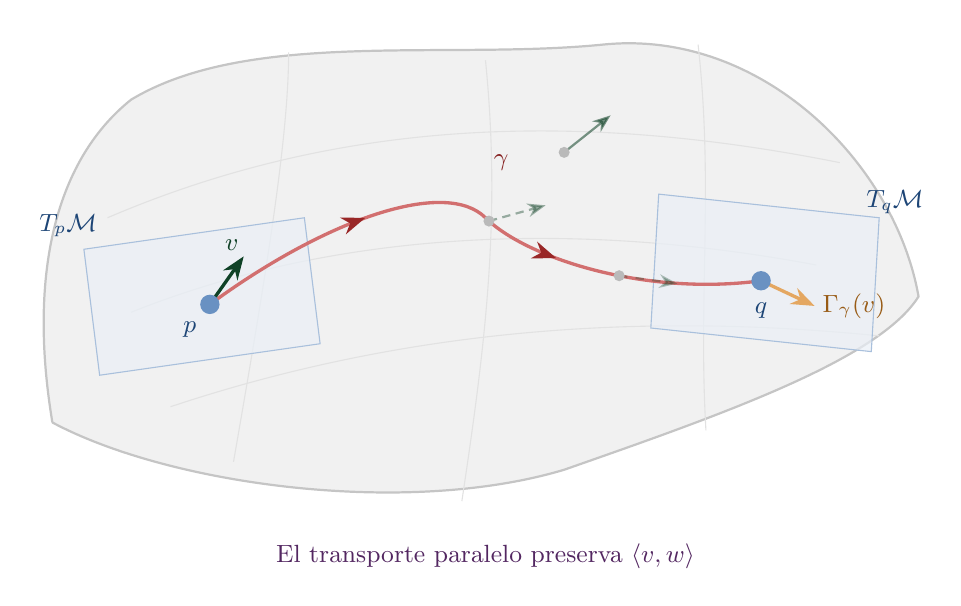
\begin{tikzpicture}[>=Stealth]

% === Superficie curva ===
\fill[gdlgray!12]
    (-5.5, -1.8) .. controls (-4, -2.6) and (-1, -3.0) .. (1, -2.4)
    .. controls (3, -1.7) and (5, -1.0) .. (5.5, -0.2)
    .. controls (5.2, 1.5) and (3.5, 3.2) .. (1.5, 3.0)
    .. controls (-0.5, 2.8) and (-3, 3.2) .. (-4.5, 2.3)
    .. controls (-5.5, 1.5) and (-5.8, 0.0) .. (-5.5, -1.8);

\draw[thick, gdlgray!50]
    (-5.5, -1.8) .. controls (-4, -2.6) and (-1, -3.0) .. (1, -2.4)
    .. controls (3, -1.7) and (5, -1.0) .. (5.5, -0.2)
    .. controls (5.2, 1.5) and (3.5, 3.2) .. (1.5, 3.0)
    .. controls (-0.5, 2.8) and (-3, 3.2) .. (-4.5, 2.3)
    .. controls (-5.5, 1.5) and (-5.8, 0.0) .. (-5.5, -1.8);

% Malla interna (curvas horizontales)
\draw[gdlgray!25, thin]
    (-4.8, 0.8) .. controls (-2, 2.0) and (1, 2.2) .. (4.5, 1.5);
\draw[gdlgray!25, thin]
    (-4.5, -0.4) .. controls (-2, 0.6) and (1, 0.8) .. (4.2, 0.2);
\draw[gdlgray!25, thin]
    (-4, -1.6) .. controls (-1, -0.6) and (2, -0.4) .. (5, -0.7);

% Malla interna (curvas verticales)
\draw[gdlgray!25, thin]
    (-3.2, -2.3) .. controls (-2.8, 0) and (-2.5, 1.8) .. (-2.5, 2.9);
\draw[gdlgray!25, thin]
    (-0.3, -2.8) .. controls (0, -0.8) and (0.2, 0.8) .. (0, 2.8);
\draw[gdlgray!25, thin]
    (2.8, -1.9) .. controls (2.7, -0.2) and (2.9, 1.2) .. (2.7, 3.0);

% === Coordenadas de p y q ===
\coordinate (p) at (-3.5, -0.3);
\coordinate (q) at (3.5, 0.0);

% === Plano tangente en p ===
\fill[gdlblue!10, opacity=0.7]
    ($(p) + (-1.4, -0.9)$) -- ($(p) + (1.4, -0.5)$)
    -- ($(p) + (1.2, 1.1)$) -- ($(p) + (-1.6, 0.7)$) -- cycle;
\draw[gdlblue!40, thin]
    ($(p) + (-1.4, -0.9)$) -- ($(p) + (1.4, -0.5)$)
    -- ($(p) + (1.2, 1.1)$) -- ($(p) + (-1.6, 0.7)$) -- cycle;
\node[gdlblue!70!black, font=\small] at ($(p) + (-1.8, 1.0)$) {$T_p\mathcal{M}$};

% === Plano tangente en q ===
\fill[gdlblue!10, opacity=0.7]
    ($(q) + (-1.4, -0.6)$) -- ($(q) + (1.4, -0.9)$)
    -- ($(q) + (1.5, 0.8)$) -- ($(q) + (-1.3, 1.1)$) -- cycle;
\draw[gdlblue!40, thin]
    ($(q) + (-1.4, -0.6)$) -- ($(q) + (1.4, -0.9)$)
    -- ($(q) + (1.5, 0.8)$) -- ($(q) + (-1.3, 1.1)$) -- cycle;
\node[gdlblue!70!black, font=\small] at ($(q) + (1.7, 1.0)$) {$T_q\mathcal{M}$};

% === Curva gamma de p a q ===
% Curva suave con cresta moderada, bien dentro de la superficie
\draw[very thick, gdlred!70,
    decoration={markings,
        % Flechas de direccion
        mark=at position 0.30 with {\arrow[gdlred!80!black, line width=0.8pt]{Stealth[length=3mm]}},
        mark=at position 0.65 with {\arrow[gdlred!80!black, line width=0.8pt]{Stealth[length=3mm]}},
        % Coordenadas intermedias exactas sobre la curva
        mark=at position 0.28 with {\coordinate (m1);},
        mark=at position 0.52 with {\coordinate (m2);},
        mark=at position 0.76 with {\coordinate (m3);}},
    postaction={decorate}]
    (p) .. controls (-2.0, 0.8) and (-0.5, 1.3) .. (0, 0.8)
    .. controls (0.5, 0.3) and (2.0, -0.2) .. (q);

% Etiqueta gamma
\node[gdlred!70!black, font=\small] at (0.2, 1.5) {$\gamma$};

% === Vector original v en p ===
% Longitud 0.75, angulo ~55 grados
\draw[->, very thick, gdlgreen!50!black] (p) -- ++(0.43, 0.61)
    node[above left=-2pt, font=\small, gdlgreen!50!black] {$v$};

% === Vectores intermedios transportados ===
% Rotacion gradual en sentido horario: ~55 -> ~40 -> ~15 -> ~-5 -> ~-25 grados
% Longitud constante ~0.75

% Intermedio 1 (t=0.28): angulo ~38 grados
\draw[->, thick, gdlgreen!50!black, opacity=0.55]
    (m1) -- ++(0.59, 0.47);

% Intermedio 2 (t=0.52): angulo ~15 grados
\draw[->, thick, gdlgreen!50!black, opacity=0.40, densely dashed]
    (m2) -- ++(0.72, 0.20);

% Intermedio 3 (t=0.76): angulo ~-8 grados
\draw[->, thick, gdlgreen!50!black, opacity=0.30, dashed]
    (m3) -- ++(0.74, -0.10);

% === Vector transportado final en q ===
% Angulo ~-25 grados, longitud 0.75
\draw[->, very thick, gdlorange!70] (q) -- ++(0.68, -0.32)
    node[right=-1pt, font=\small, gdlorange!70!black] {$\Gamma_\gamma(v)$};

% === Puntos p y q (encima de todo) ===
\fill[gdlblue!70] (p) circle (3.5pt);
\node[below left, font=\small, gdlblue!70!black] at ($(p) + (-0.05, -0.1)$) {$p$};

\fill[gdlblue!70] (q) circle (3.5pt);
\node[below, font=\small, gdlblue!70!black] at ($(q) + (0, -0.15)$) {$q$};

% Puntos intermedios
\fill[gdlgray!60] (m1) circle (2pt);
\fill[gdlgray!60] (m2) circle (2pt);
\fill[gdlgray!60] (m3) circle (2pt);

% === Nota sobre preservacion del producto interno ===
\node[font=\small, text=gdlpurple!70!black] at (0, -3.5) {
    El transporte paralelo preserva $\langle v, w \rangle$
};

\end{tikzpicture}
\end{document}
